\documentclass[12pt]{article}
\usepackage[margin=1in]{geometry} 
\geometry{
 a4paper,
 total={170mm,257mm},
 left=15mm,
 right=15mm,
 top=16mm,
 bottom = 15mm
 }
\usepackage{amsmath,amsthm,amssymb}
\usepackage{graphicx}
\usepackage{array}
\usepackage[table,xcdraw]{xcolor}
\usepackage{titling}
\usepackage{subcaption}
\usepackage[export]{adjustbox}
\usepackage{float}
\usepackage{amsmath}


\begin{document}


% \setlength{\droptitle}{-6em}     % Eliminate the default vertical space
% \addtolength{\droptitle}{-4pt} 

\title{Term Paper }
\author{MA473}
% \vspace{-4cm}
\date{Akshat Gupta - 180123002 \\
Ashish Barnawal - 180123006\\
Karan Gupta - 180123064
}
\maketitle

\section{Introduction}

\hspace{.5cm} Based on the following assumptions Black and Scholes derived the Black Scholes formula

\begin{enumerate}
    \item The asset price follows geometric Brownian motion i.e. $d S=\mu S d t+\sigma S d W$.

\item The risk-free interest rate is $\mathrm{r}$ is constant until expiration date.

\item Investors can borrow and lend at risk-free rates.
\item The stock doesn't pay dividends.

\item The market is frictionless (no tax/transaction costs and all securities are divisible).

\item No risk-free arbitrage opportunity exists.

\item Security trading is continuous.

\item Option is a European option.
\end{enumerate}

Based on above, the Black-Scholes PDE is given by:

$$
\frac{\partial V}{\partial t}+\frac{1}{2} \sigma^{2} S^{2} \frac{\partial^{2} V}{\partial S^{2}}+r S \frac{\partial V}{\partial S}-r V=0.
$$

with terminal conditions:

\begin{enumerate}
    \item For European call option:
    
    \begin{align*}
    V(0, t)&=0 & \lim _{S \rightarrow+\infty} V(S, t)&=S & V(S, T)&=\max (S-K, 0)
    \end{align*}

    

\item For European put option

    \begin{align*}
        V(0, t)&=K e^{-r(T-t)} & \lim _{S \rightarrow+\infty} V(S, t)&=0 & V(S, T)&=\max (K-S, 0)
    \end{align*}

\end{enumerate}

The solution can be found analytically to be:

\begin{enumerate}
    \item For European call: $V(S, t)=S N\left(d_{1}\right)-K N\left(d_{2}\right) e^{-r(T-t)}$
    
    \item For European put: $V(S, t)=S N\left(-d_{2}\right) e^{-r(T-t)}-S N\left(-d_{1}\right)$
\end{enumerate}


where,

$$
\begin{gathered}
N(x)=\frac{1}{\sqrt{2 \pi}} \int_{-\infty}^{x} e^{-\frac{y^{2}}{2}} d y \\
d_{1}=\frac{\log \left(\frac{S}{K}\right)+\left(r+\frac{1}{2} \sigma^{2}\right)(T-t)}{\sigma \sqrt{T-t}} \\
d_{2}=\frac{\log \left(\frac{S}{K}\right)+\left(r-\frac{1}{2} \sigma^{2}\right)(T-t)}{\sigma \sqrt{T-t}}
\end{gathered}
$$



\section{Space discretization}

\subsection{Fourth order central finite difference}

We write the formula as:

$$
\frac{\partial V}{\partial S}=A V+b_{1} \quad \quad \frac{\partial^{2} V}{\partial S^{2}}=B V+b_{2}
$$

where

$$
\begin{gathered}
A=\frac{1}{12 h}\left[\begin{array}{cccccc}
-10 & 18 & -6 & 1 & & \\
-8 & 0 & 8 & -1 & & \\
1 & -8 & 0 & 8 & & \\
& & \ddots & \ddots & \ddots & \\
& & 1 & \ldots & 0 & 8 \\
& & 1 & -6 & 18 & -10
\end{array}\right] \quad B=\frac{1}{12 h^{2}}\left[\begin{array}{cccccc}
-15 & -4 & 14 & -6 & 1 & \\
16 & -30 & 16 & -1 & & \\
-1 & 16 & -30 & 16 & \ddots & \\
& & & \ddots & \ddots & \\
& & -4 & \cdots & -30 & 16\\
& 1 & -6 & 14 & -4 & -15
\end{array}\right]
\end{gathered}
$$

$$b_{1}=\frac{1}{12 h}\left(-3 V_{0} \quad V_{0} \quad 0 \quad \cdots \quad -V_{N} \quad -3 V_{N}\right)^{T}$$ 
$$b_{2}=\frac{1}{12 h^{2}}\left(10 V_{0} \quad -V_{0} \quad 0 \quad \cdots \quad -V_{N} \quad 10 V_{N}\right)^{T}$$

Thus the BS PDE can be written as

$$
\frac{d V}{d t}=-P V-Q \text { where } P=\frac{1}{2} \sigma^{2} S^{2} B+r S A-r I \text { and } Q=\frac{1}{2} \sigma^{2} S^{2} b_{2}+r S b_{1}
$$

\subsection{Fourth order compact finite difference scheme}

$$
\frac{\partial V}{\partial t}=-L V
$$

where

$$
\begin{aligned}
L &=\frac{1}{2} \sigma^{2} S^{2} D^{2}+r S D-r I \\
D &=F^{-1} G \\
D^{2} &=U^{-1} W
\end{aligned}
$$



$$
F=\left[\begin{array}{ccccc}
1 & 3 & 0 & & \\
\frac{1}{4} & 1 & \frac{1}{4} & & \\
& \ddots & \ddots & \ddots & \\
& & \frac{1}{4} & 1 & \frac{1}{4} \\
& & 0 & 3 & 1
\end{array}\right] \quad G=\left[\begin{array}{ccccccc}
-\frac{17}{6 h} & \frac{3}{2 h} & \frac{3}{2 h} & -\frac{1}{6 h} & & \\
-\frac{3}{4 h} & 0 & \frac{3}{4 h} & & & \\
& -\frac{3}{4 h} & 0 & \frac{3}{4 h} & & \\
& & \ddots & \ddots & & \\
&  & & & -\frac{3}{4 h} & 0 & \frac{3}{4 h} \\
 & & & \frac{1}{6 h} & -\frac{3}{2 h} & -\frac{3}{2 h} & \frac{17}{6 h}
\end{array}\right]
$$

and

$$
U=\left[\begin{array}{cccccc}
1 & 10 & 0 & & & \\
\frac{1}{10} & 1 & \frac{1}{10} & & & \\
& \frac{1}{10} & 1 & \ddots & & \\
& & \ddots & \ddots & \ddots & \\
& & & \ddots & 1 & \frac{1}{10} \\
& & & 0 & 10 & 1
\end{array}\right]
$$

$$
\mathrm{W}=\left[\begin{array}{cccccc}
\frac{145}{12 h^{2}} & -\frac{76}{3 h^{2}} & \frac{29}{2 h^{2}} & -\frac{4}{3 h^{2}} & \frac{1}{12 h^{2}} & \\
\frac{6}{5 h^{2}} & -\frac{12}{5 h^{2}} & \frac{6}{5 h^{2}} & & & \\
& \ddots & \ddots & \ddots & & \\
& & \ddots & \ddots & \ddots & \\
& & & \frac{6}{5 h^{2}} & -\frac{12}{5 h^{2}} & \frac{6}{5 h^{2}} \\
& \frac{1}{12 h^{2}} & -\frac{4}{3 h^{2}} & \frac{29}{2 h^{2}} & -\frac{76}{3 h^{2}} & \frac{145}{12 h^{2}}
\end{array}\right]
$$

\section{Time discretization}

\subsection{Crank Nicolson method}

$$
\begin{aligned}
&\text { For } \frac{\partial V}{\partial t}=A V+b \\
&\left(I-\frac{\delta A}{2}\right) V^{(j+1)}=\left(I+\frac{\delta A}{2}\right) V^{(j)}+b
\end{aligned}
$$

\subsection{BDF4 method}

For $\frac{d u}{d t}=A u+b$, the scheme is given by

$$
\left(\frac{25}{12} I-\delta A\right) u^{(j+1)}=4 u^{(j)}-3 u^{(j-1)}+\frac{4}{3} u^{(j-2)}-\frac{1}{4} u^{(j-3)}+\delta b^{(j+1)}
$$



\subsection{Grid refinement}

Transform

$$
\begin{gathered}
y=\psi(S)=\frac{\sinh ^{-1}(\xi(S-K))-c_{1}}{c_{2}-c_{1}} \\
\left.S=\psi^{-1}(y)=\varphi(y)=\frac{1}{\xi} \sinh \left(c_{2} y+c_{1}(1-y)\right)+K
\end{gathered}
$$

where

$$
c_{1}=\sinh ^{-1}\left(\xi\left(S_{\min }-K\right)\right) \quad \quad c_{2}=\sinh ^{-1}\left(\xi\left(S_{\max }-K\right)\right)
$$

The Black-Scholes PDE transforms to:

$$
\frac{\partial V}{\partial t}=\frac{1}{2} \sigma^{2} \frac{\varphi(y)^{2}}{J(y)^{2}} \frac{\partial^{2} V}{\partial y^{2}}+\left(r \frac{\varphi(y)}{J(y)}-\frac{1}{2} \sigma^{2} \frac{\varphi(y)^{2}}{J(y)^{3}} H(y)\right) \frac{\partial V}{\partial y}-r V
$$

\section{Results}

\subsection{Compact Finite Difference + BDF4}

\begin{center}
    \begin{tabular}{|l|l|l|}
\hline Grid Size & Error & Order \\
\hline $10 \times 10$ & $0.031667$ & \\
\hline $20 \times 20$ & $0.009247$ & $1.775868$ \\
\hline $40 \times 40$ & $0.000782$ & $3.563366$ \\
\hline
\end{tabular}
\end{center}

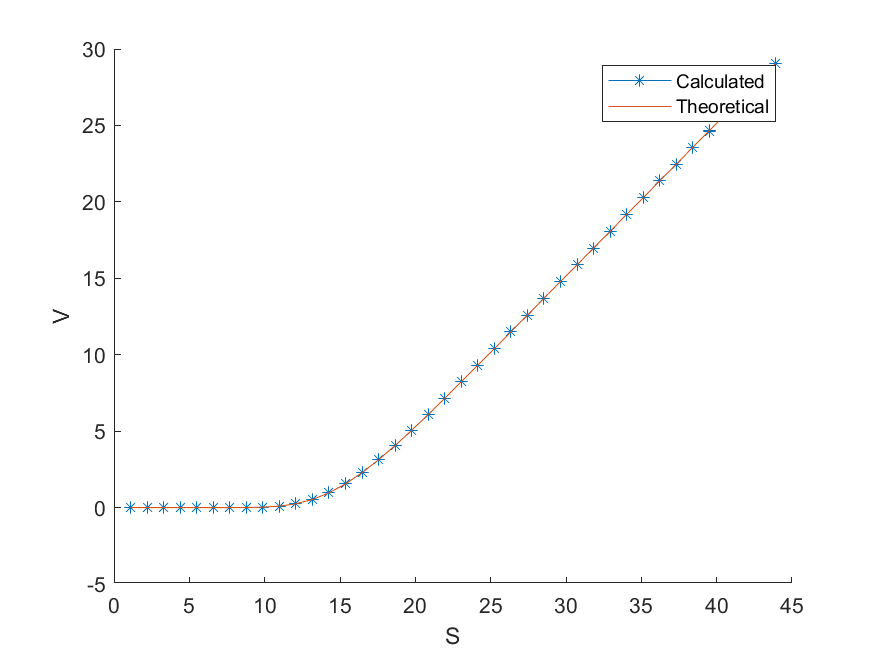
\includegraphics[scale=0.6]{comp_bdf4.png}
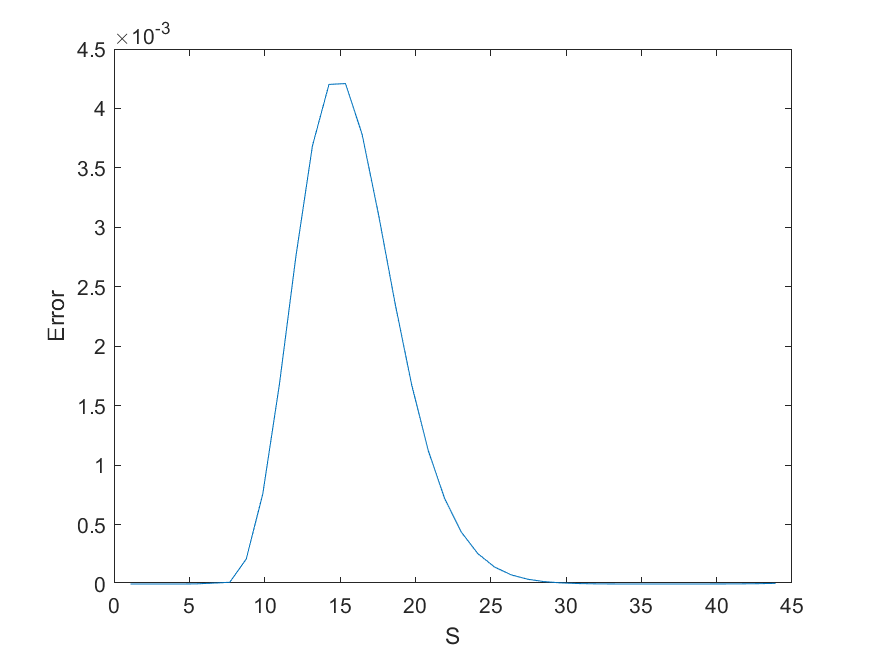
\includegraphics[scale=0.6]{comp_bdf4_e.png}

\subsection{Compact Finite Difference + Crank Nicolson}

\begin{center}
    \begin{tabular}{|l|l|l|}
\hline Grid Size & Error & Order \\
\hline $10 \times 10$ & $0.032057$ & \\
\hline $20 \times 20$ & $0.009247$ & $1.793653$ \\
\hline $40 \times 40$ & $0.000782$ & $3.563347$ \\
\hline
\end{tabular}
\end{center}


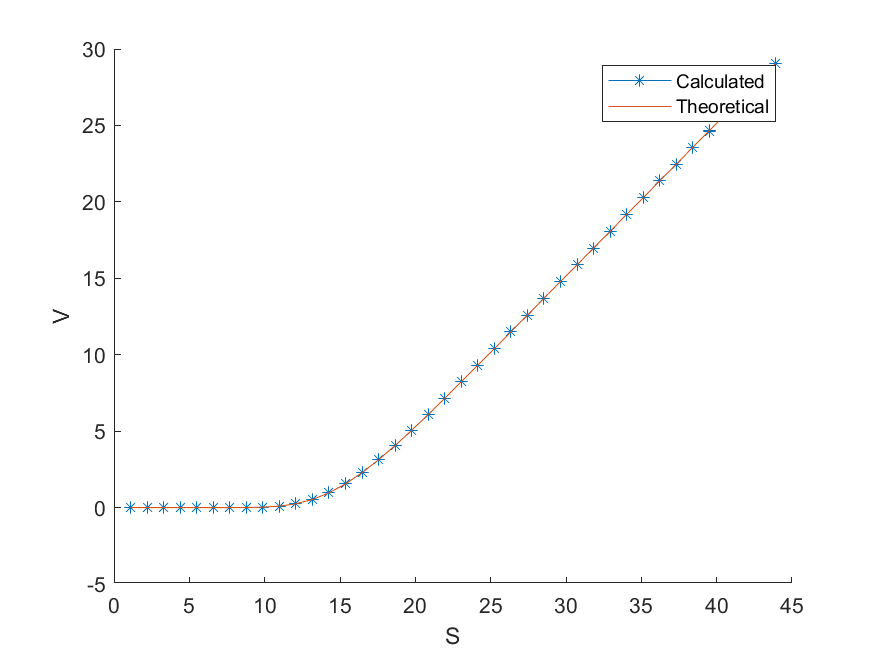
\includegraphics[scale=0.6]{comp_cn.png}
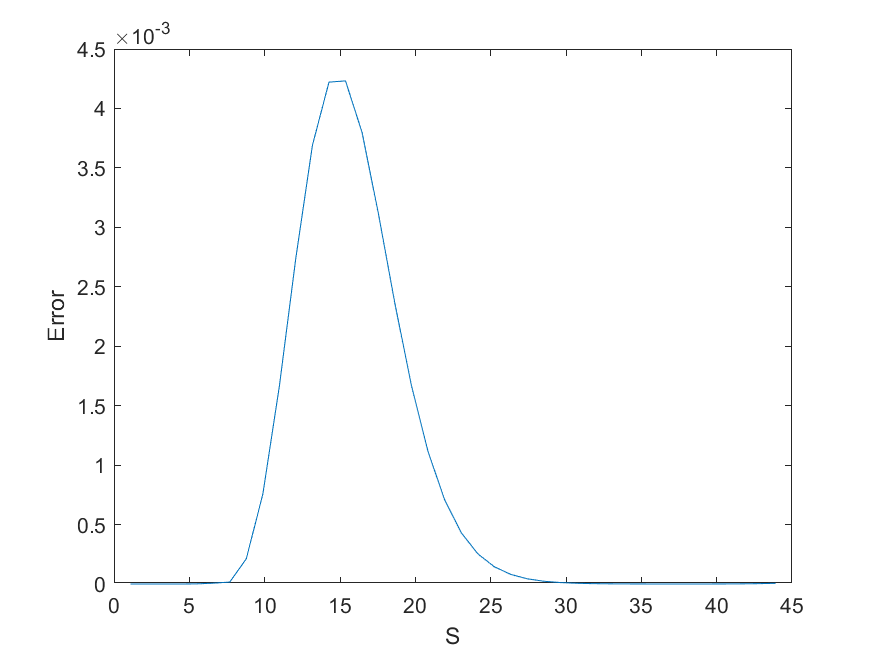
\includegraphics[scale=0.6]{comp_cn_e.png}

\subsection{Finite Difference + Crank Nicolson + Grid Refinement} 


\begin{center}
    \begin{tabular}{|l|l|l|}
\hline Grid Size & Error & Order \\
\hline $10 \times 10$ & $0.017660$ & \\
\hline $20 \times 20$ & $0.005036$ & $1.810200$ \\
\hline $40 \times 40$ & $0.000613$ & $3.039027$ \\
\hline
\end{tabular}
\end{center}

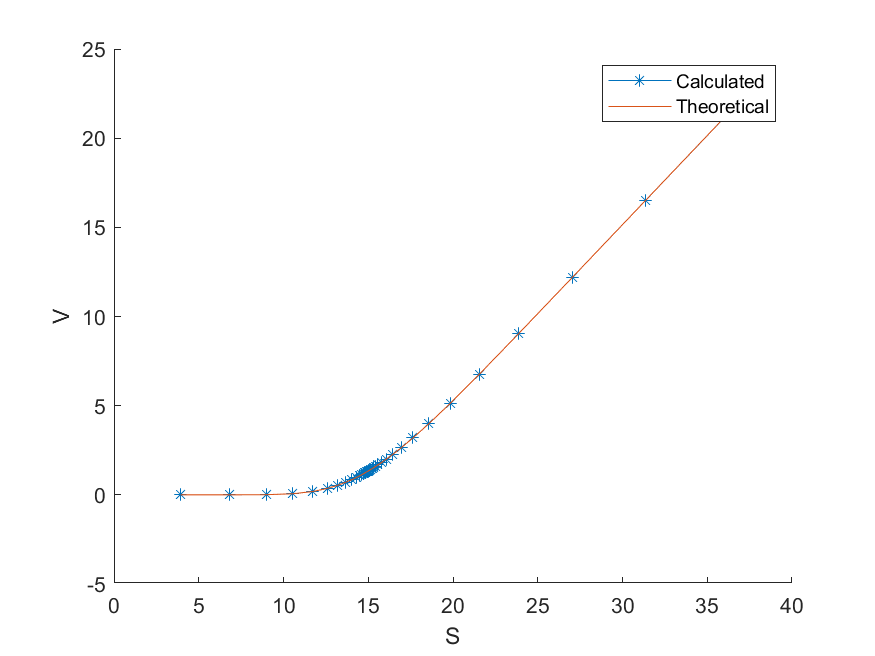
\includegraphics[scale=0.6]{comp_cn_gr.png}
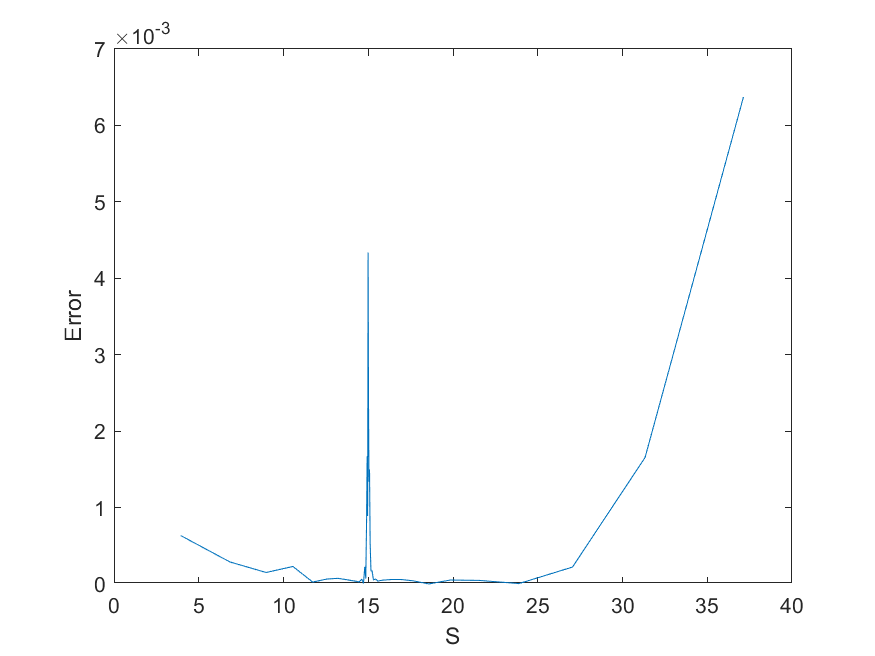
\includegraphics[scale=0.6]{comp_cn_gr_e.png}

\subsection{Compact Finite Difference + BDF4 + Grid Refinement}

\begin{center}
    \begin{tabular}{|l|l|l|}
\hline Grid Size & Error & Order \\
\hline $10 \times 10$ & $0.015779$ & \\
\hline $20 \times 20$ & $0.003903$ & $2.015336$ \\
\hline $40 \times 40$ & $0.000256$ & $3.930728$ \\
\hline
\end{tabular}
\end{center}

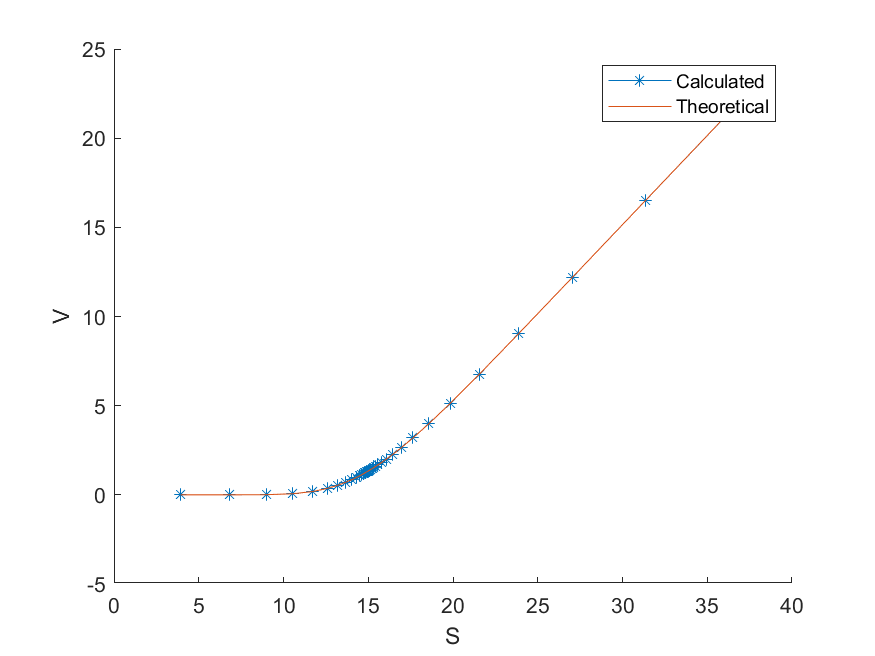
\includegraphics[scale=0.6]{comp_bdf4_gr.png}
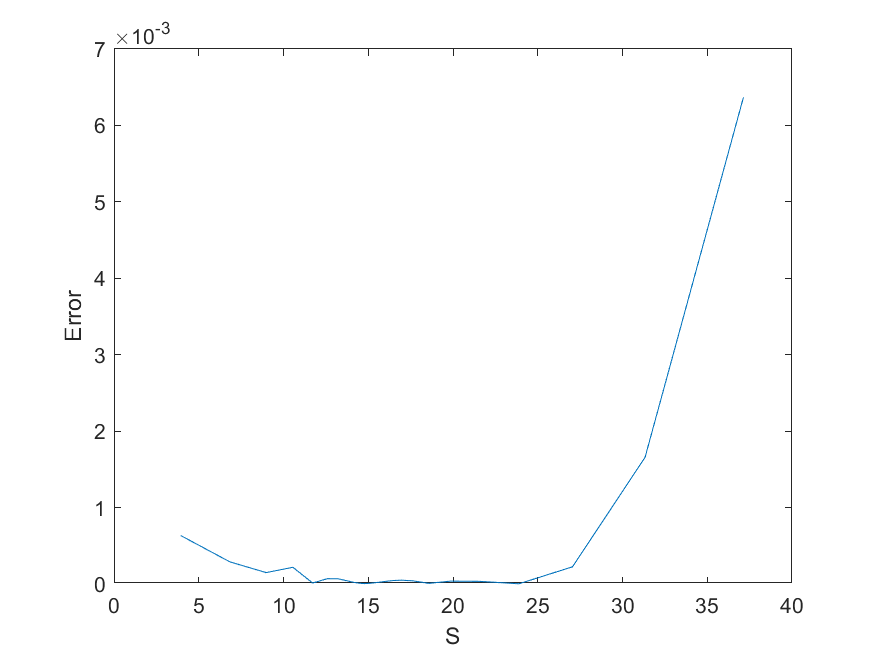
\includegraphics[scale=0.6]{comp_bdf4_gr_e.png}

\end{document}
